\documentclass{standalone}
\usepackage{tikz}
\usepackage{amssymb}

\begin{document}

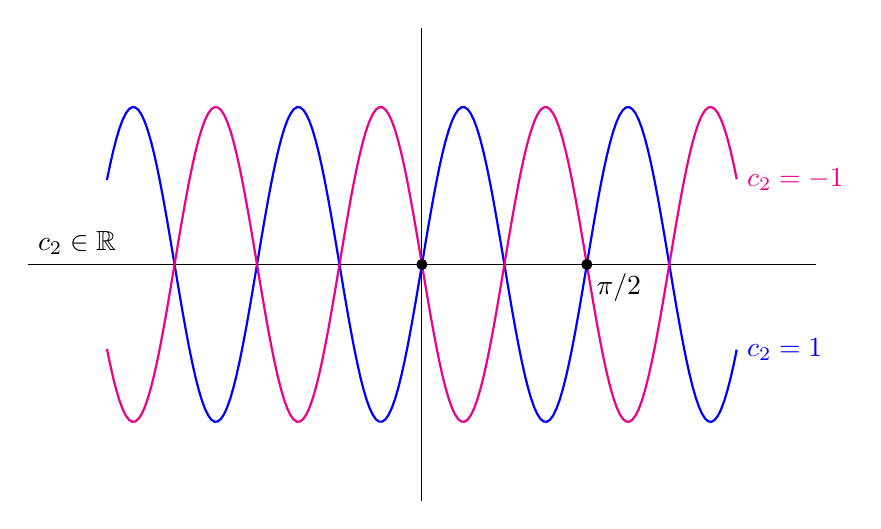
\begin{tikzpicture}[>=latex]
	\draw (-5,0) node [above right] { \(c_2 \in \mathbb{R}\)} -- (5,0) (0,-3) -- (0,3);
	\draw [blue,    thick, domain=-4:4, samples = 200] plot(\x , {2*sin(3*\x r)}) node [right] { \(c_2=1\)};
	\draw [magenta ,thick, domain=-4:4, samples = 200] plot(\x , {-2*sin(3*\x r)}) node [right] { \(c_2=-1\)};
	\fill (0,0) circle (2pt);
	\fill (2*pi/3,0) circle (2pt) node [below right] { \(\pi /2\)};
\end{tikzpicture}

\end{document}
